\section{Simulation Results}\label{sec:results}

The proposed method was implemented in C++ and tested
using a \SI[mode=text]{3.20}{\GHz} CPU with 
\SI{8}{GB} memory.  We demonstrate the results using 
three applications executed by three biochips.
The information of these test cases are shown in 
Table~\ref{tb_test}, where IVD (In-Vitro Diagnostics),
PID (Protein Interpolation Dilution) and 
CPA (Colorimetric Protein Assay)
are real-world assays. The biochips used in the experiments were
the IVD chip and RA30 chip from \cite{Liu2017} and 
the mRNA chip from \cite{MAQuake06}. 
%In the experiments, we used Gurobi \cite{gurobi} to solve the optimization problems.

In Table~\ref{tb_test}, the results of DFT design of the chips above running
the three applications are reported, where all chips have been modified 
to single-source single-meter architectures successfully.
For each chip-application combination, the results are
split into two rows, each of which contain three columns. In the first row,
the number of added DFT valves, the number of the valves sharing control
channels with existing valves and the runtime of the proposed method are
shown. For all the combinations, the DFT valves have found a valid sharing
mechanism. Compared with the number of original valves in the chips, the
number of DFT valves is still in the acceptable range. The second row for 
an experiment combination reports the execution time of the corresponding
application without DFT, with DFT but without PSO optimization for valve 
sharing and the final result of the whole framework. From this comparison,
it can be seen that the introduction of DFT valves into a chip can initially
prolong the execution time of an application significantly. With 
PSO optimization iterations, the execution time has been recovered back to
nearly the same level of the original design, while in the case PID running on
the RA30 chip the execution time has actually been reduced.

%The column $t_b$ shows at the beginning
%of PSO, the best running time of assays executed on DFT architecures. The
%execution time after is presented in column $t_a$. As we can see, relative to
%execution time before optimization, assays acheive less running time after
%PSO. But they are still longer than the execution time when applications
%running on the original chips. This is due to valve sharing interference with
%flow paths during the execution, leading more waiting time among the fluid
%traffics.  The execution time for the whole program is record in column $t_p$.


\begin{table*}[t] 
\footnotesize
\centering
\renewcommand{\tabcolsep}{7.35pt}
\renewcommand{\arraystretch}{1}
\caption{Results of Test Pattern Generation with Single Pressure Source and Single Pressure Sensor}
\label{tb_test}
\begin{tabular}{cr r ccccccc r ccccccc} \hlinewd{0.7pt}
\multicolumn{2}{c}{FPVA} &
\multicolumn{1}{c}{} &
\multicolumn{7}{c}{Direct Approach} &
\multicolumn{1}{c}{} &
\multicolumn{7}{c}{Loop Acceleration} \\
\cline {1-2}\cline {4-10}\cline {12-18} 
\multicolumn{1}{c}{Dimension} &
\multicolumn{1}{c}{$n_v$} &
\multicolumn{1}{c}{} &
\multicolumn{1}{c}{$n^d_p$} &
\multicolumn{1}{c}{$t^d_p(s)$} &
\multicolumn{1}{c}{$n^d_c$} &
\multicolumn{1}{c}{$t^d_c(s)$} &
\multicolumn{1}{c}{$n^d_l$} &
\multicolumn{1}{c}{$t^d_l(s)$} &
\multicolumn{1}{c}{$N^d$} &
% \multicolumn{1}{c}{$T^d(s)$} &
\multicolumn{1}{c}{} &
\multicolumn{1}{c}{$n^a_p$} &
\multicolumn{1}{c}{$t^a_p(s)$} &
\multicolumn{1}{c}{$n^a_c$} &
\multicolumn{1}{c}{$t^a_c(s)$} &
\multicolumn{1}{c}{$n^a_l$} &
\multicolumn{1}{c}{$t^a_l(s)$} &
\multicolumn{1}{c}{$N^a$} \\
% \multicolumn{1}{c}{$T^a(s)$} \\


\hlinewd{0.6pt}

5 $\times$5 &40&&2	&0.02	&8	&0.67	&3	&0.01	&13	&&2	&0.02	&8	&0.16	&3	&0.02	&13	\\
10$\times$10&380&&2	&0.72	&18	&46	&3	&0.04	&23	&&2	&2.61	&18	&12	&3	&0.03	&23	\\
15$\times$15&420&&2	&48	&28	&984	&4	&0.12	&34	&&2
	    &78	&28	&40	&3      &73	&33	   	\\
20$\times$20&760&&2	&758	&*	&*	&*	&*	&*	&&2	&363	&38	&146	&3	&163	&43	\\
25$\times$25&1200&&*	&*	&*	&*	&*	&*	&*	&&3	&1200	&48	&472	&3	&966	&54	\\
30$\times$30&1740&&*	&*	&*	&*	&*	&*	&*	&&3	&1201	&58	&1648	&4	&1243	&65	\\

% 5  $\times$ 5   &39  &&1 $\times$  1&5 $\times$ 5  &&5  & 0.3  &&8  &0.2 & &  4  &  2   &&17 & 2.5 \\ 
% 10 $\times$ 10  &176 &&2 $\times$  2&5 $\times$ 5  &&4  & 4    &&18 &5   & &  4  &  10  &&26 & 19  \\
% 15 $\times$ 15  &411 &&3 $\times$  3&5 $\times$ 5  &&8  & 17   &&28 &26  & &  8  &  127 &&44 & 170 \\
% 20 $\times$ 20  &744 &&4 $\times$  4&5 $\times$ 5  &&16 & 35   &&38 &41  & & 16  & 742  &&70 & 818 \\
% 30 $\times$ 30  &1704&&6 $\times$  6&5 $\times$ 5  &&20 & 255  &&58 &171 & & 20  & 1492 &&98 & 1918\\
\hlinewd{0.7pt}
\multicolumn{18}{l}{* -- No valid result}\\
\end{tabular}
\end{table*}





\begin{figure}[t]
{
\figurefontsize
\centering
%\vskip 5pt
\pgfplotsset{compat=1.3,
    %legend drawing style, single bar instead of the default double mini bars
    /pgfplots/ybar legend/.append style={ 
        /pgfplots/legend image code/.code={%
           \draw[##1,/tikz/.cd,yshift=-0.25em]
           (0cm,0cm) rectangle (7pt,0.8em);
        },
    }
}

%%sharp linear plots
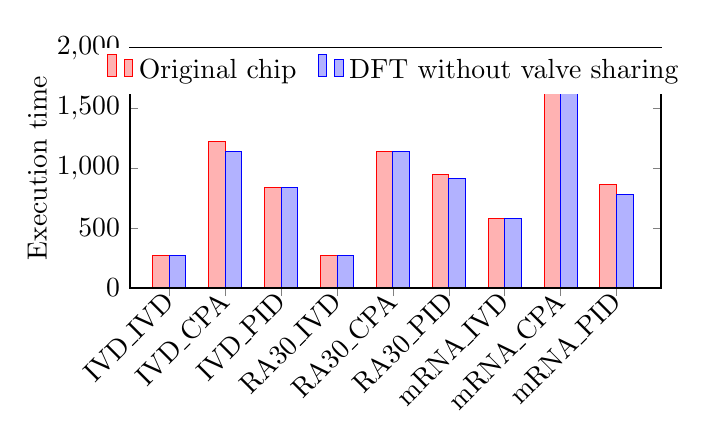
\begin{tikzpicture}
%remove space surrounding text nodes and the whole picture caused by text
%[every node/.style={inner sep=0,outer sep=0}]

%\pgfplotstableread{
%$chip  timebefore  timeafter
%1        9         25          
%2        62        103            
%3        51        168            
%4        43         90            
%5        74        137            
%6        95        171          
%7        102       140            
%8        107       160
%9        174       214
%10       138       256
            
%}\loadedtable

\pgfplotstableread{
chip timebefore timeafter
1 270	270
2 1220	1140
3 840	840
4 270	270
5 1140	1140
6 950	910
7 580	580
8 1640	1640
9 860	780




}\loadedtable

\begin{axis}[
%xaxis styles
%xticklabels={s5378,s9234, s13207, s15850, s38584,systemcdes, mem\_ctrl, usb\_funct, ac97\_ctr, pci\_bridge32}, 
xticklabels={IVD\_IVD, IVD\_CPA, IVD\_PID, RA30\_IVD,RA30\_CPA, RA30\_PID, mRNA\_IVD, mRNA\_CPA, mRNA\_PID}, 
xtick={1,...,9},
%x axis limits
xmin=0.3, xmax=9.8,
%x and y axes scaling
%x=0.763cm, y=0.18cm,
x=0.71cm, y=0.0152mm, 
x tick label style={rotate=45, xshift=0pt,yshift=0pt,anchor=east, 
%"iner sep" removes the space surrounding label tick texts at the bottom,
%so that there is no useless white space at the lower boundary of the picture. The
%space of tick label texts need to be removed because they are the lowest
%units without an xlable
inner sep=0}, 
xticklabel pos=left, xtick align=outside, xtick pos=left,
%
%y axis limits
ymin=0, ymax=2000,
%yaxis styles
ylabel={Execution time}, 
%"inner sep" for ylabel removes the white space on the leftmost edge of the picture
ylabel style={inner sep=0}, 
ylabel shift=0pt, ytickmin=0,ytickmax=2000, 
%
%legend styles
legend columns=3, 
legend style={
at={(0.5,0.907)}, anchor=center, 
%column separation between legend items
/tikz/every even column/.append style={column sep=0.2cm},
%distance between legend symbols and text nodes
%column sep=2.5cm,
%space surrounding the text boxes in legend
%nodes={inner xsep=20pt},
%no stroke in legend
draw=none, 
},
%
%axis drawing line width
line width=0.75pt,
%space between the bars in a group
ybar=0pt, 
bar width=6pt,
%axis on top makes the bars drawn on a layer below axis lines. Otherwise, the bottom lines of the
%bars can be seen with different colors on the bottom axis line.
axis on top=true,
major tick length=3pt,
]  
\addplot[ybar, line width=0.35pt, red, fill=red!30!white] table[x=chip,y=timebefore] {\loadedtable};
%\addplot[ybar, line width=0.35pt, brown!60!black, fill=brown!30!white] table[x=chip,y=Multiplex] {\loadedtable};
\addplot[ybar, line width=0.35pt, blue, fill=blue!30!white] table[x=chip,y=timeafter] {\loadedtable};
\legend{Original chip, DFT without valve sharing}

\end{axis}
\end{tikzpicture}

%\begin{tikzpicture}
\begin{axis}[
x=1.1cm, y=0.27cm, ymax=12, line width=0.75pt,
ylabel={Channel (Valve) Ratio}, ylabel shift=-6pt, 
xtick={1,...,6},xticklabels={RA100, RA70, CPA, RA30, IVD, PCR},
x tick label style={rotate=330, xshift=-15pt,yshift=-5pt,anchor=west}, 
xticklabel pos=left, xtick align=outside, xtick pos=left,
ytickmin=0,ytickmax=10, 
ytick={0,5,10}, yticklabels={0,0.5,1},
legend columns=2, legend style={at={(0.5,0.9)}, anchor=center, nodes={inner xsep=2pt},
draw=none, column sep=1pt},
ybar=0pt, bar width=7
]
   \addplot[line width=0.5pt, black, fill=orange!70!white] table[x=cir,y=edge] 
{edge_valve_percentage.dat};
   \addplot[line width=0.5pt, black, fill=blue!65!orange] table[x=cir,y=valve] 
{edge_valve_percentage.dat};

   \legend{Channel\hspace*{8pt}, Valve\hspace*{8pt}}
\end{axis}
\end{tikzpicture}

\caption{Comparison of execution time of applications 
using original chips and DFT architectures without valve sharing.}
\label{fig:exetime_cmp}
}
\end{figure}


As shown in Table~\ref{tb_test}, the execution time of applications is slightly
longer in many cases with DFT architectures than with the original chip.  The
main reason is that valve sharing blocks some transportation tasks so that
operations must wait for fluid samples. In the case that the DFT
valves can have their own control channels, the execution time should be no
larger than that in the original chip, because new resources added for DFT can
also be used by applications.  The results of this comparison are shown in
\figname~\ref{fig:exetime_cmp}, where the execution performance is better in
several cases.

In the DFT architectures, the number of pressure sources and meters have been
reduced. Accordingly, the number of test vectors should increase because some
test vectors become unavailable with this simplified test platform.
Figure~\ref{fig:testvector_cmp} compares the numbers of test vectors in the
original chips and the DFT architectures.  The larger number of test vectors
leads to a relatively longer test time, which is still not a problem in today's biochemical
laboratories. 

In the process of PSO optimization, we used 5 particles for DFT valves and
channels and 5 particles for valve sharing. The total number of iterations was
set to 100. To show the converging trend of the PSO method, the execution times
of applications with respect to the number of iterations are shown in 
\figname~\ref{fig:PSO_iteration} for three chip-application combinations,
where we can see that the results of PSO become stable at about 80 iterations,
earlier than the number of iterations we used in the experiments.

\begin{figure}[t]
{
\figurefontsize
\centering
%\vskip 5pt
\pgfplotsset{compat=1.3,
    %legend drawing style, single bar instead of the default double mini bars
    /pgfplots/ybar legend/.append style={ 
        /pgfplots/legend image code/.code={%
           \draw[##1,/tikz/.cd,yshift=-0.25em]
           (0cm,0cm) rectangle (7pt,0.8em);
        },
    }
}

%%sharp linear plots
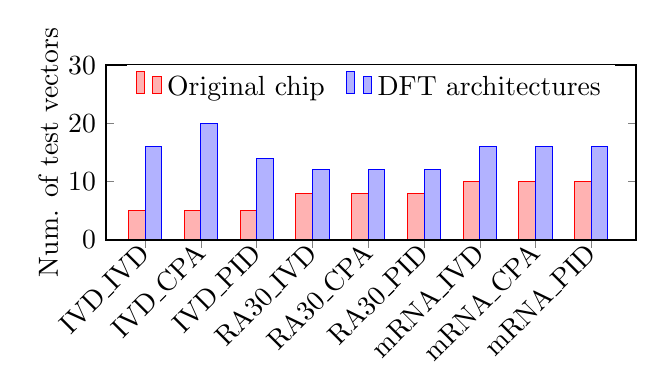
\begin{tikzpicture}
%remove space surrounding text nodes and the whole picture caused by text
%[every node/.style={inner sep=0,outer sep=0}]

%\pgfplotstableread{
%$chip  testVbefore  timeVafter
%1        9         25          
%2        62        103            
%3        51        168            
%4        43         90            
%5        74        137            
%6        95        171          
%7        102       140            
%8        107       160
%9        174       214
%10       138       256
            
%}\loadedtable

\pgfplotstableread{
chip testVbefore timeVafter
1 5	16
2 5	20
3 5	14
4 8	12
5 8	12
6 8	12
7 10	16
8 10	16
9 10	16
}\loadedtable

\begin{axis}[
%xaxis styles
%xticklabels={s5378,s9234, s13207, s15850, s38584,systemcdes, mem\_ctrl, usb\_funct, ac97\_ctr, pci\_bridge32}, 
xticklabels={IVD\_IVD, IVD\_CPA, IVD\_PID, RA30\_IVD,RA30\_CPA, RA30\_PID, mRNA\_IVD, mRNA\_CPA, mRNA\_PID}, 
xtick={1,...,9},
%x axis limits
xmin=0.3, xmax=9.8,
%x and y axes scaling
%x=0.763cm, y=0.18cm,
x=0.708235cm, y=0.0738cm, 
x tick label style={rotate=45, xshift=0pt,yshift=0pt,anchor=east, 
%"iner sep" removes the space surrounding label tick texts at the bottom,
%so that there is no useless white space at the lower boundary of the picture. The
%space of tick label texts need to be removed because they are the lowest
%units without an xlable
inner sep=0}, 
xticklabel pos=left, xtick align=outside, xtick pos=left,
%
%y axis limits
ymin=0, ymax=30,
%yaxis styles
ylabel={Num. of test vectors}, 
%"inner sep" for ylabel removes the white space on the leftmost edge of the picture
ylabel style={inner sep=0}, 
ylabel shift=0pt, ytickmin=0,ytickmax=30, 
%
%legend styles
legend columns=3, 
legend style={
at={(0.5,0.87)}, anchor=center, 
%column separation between legend items
/tikz/every even column/.append style={column sep=0.2cm},
%distance between legend symbols and text nodes
%column sep=2.5cm,
%space surrounding the text boxes in legend
%nodes={inner xsep=20pt},
%no stroke in legend
draw=none, 
},
%
%axis drawing line width
line width=0.75pt,
%space between the bars in a group
ybar=0pt, 
bar width=6pt,
%axis on top makes the bars drawn on a layer below axis lines. Otherwise, the bottom lines of the
%bars can be seen with different colors on the bottom axis line.
axis on top=true,
major tick length=3pt,
]  
\addplot[ybar, line width=0.35pt, red, fill=red!30!white] table[x=chip,y=testVbefore] {\loadedtable};
%\addplot[ybar, line width=0.35pt, brown!60!black, fill=brown!30!white] table[x=chip,y=Multiplex] {\loadedtable};
\addplot[ybar, line width=0.35pt, blue, fill=blue!30!white] table[x=chip,y=timeVafter] {\loadedtable};
\legend{Original chip, DFT architectures}

\end{axis}

% used to align with other figures
\draw[white] (-0.98,0) circle (0.01);

\end{tikzpicture}

%\begin{tikzpicture}
\begin{axis}[
x=1.1cm, y=0.27cm, ymax=12, line width=0.75pt,
ylabel={Channel (Valve) Ratio}, ylabel shift=-6pt, 
xtick={1,...,6},xticklabels={RA100, RA70, CPA, RA30, IVD, PCR},
x tick label style={rotate=330, xshift=-15pt,yshift=-5pt,anchor=west}, 
xticklabel pos=left, xtick align=outside, xtick pos=left,
ytickmin=0,ytickmax=10, 
ytick={0,5,10}, yticklabels={0,0.5,1},
legend columns=2, legend style={at={(0.5,0.9)}, anchor=center, nodes={inner xsep=2pt},
draw=none, column sep=1pt},
ybar=0pt, bar width=7
]
   \addplot[line width=0.5pt, black, fill=orange!70!white] table[x=cir,y=edge] 
{edge_valve_percentage.dat};
   \addplot[line width=0.5pt, black, fill=blue!65!orange] table[x=cir,y=valve] 
{edge_valve_percentage.dat};

   \legend{Channel\hspace*{8pt}, Valve\hspace*{8pt}}
\end{axis}
\end{tikzpicture}

\caption{Comparison of numbers of test vectors 
  in original chips and DFT architectures.} 
  \label{fig:testvector_cmp}
}
\end{figure}

\begin{figure}[t]
{
  \figurefontsize
\centering
%\vskip 5pt
\pgfplotsset{compat=1.3,
    %legend drawing style, single bar instead of the default double mini bars
    /pgfplots/ybar legend/.append style={ 
        /pgfplots/legend image code/.code={%
           \draw[##1,/tikz/.cd,yshift=-0.25em]
           (0cm,0cm) rectangle (5pt,0.8em);
        },
    }
}

%%sharp linear plots
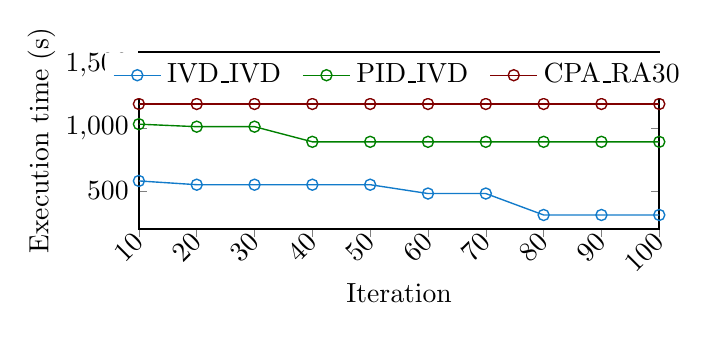
\begin{tikzpicture}
%remove space surrounding text nodes and the whole picture caused by text
%[every node/.style={inner sep=0,outer sep=0}]

%\pgfplotstableread{
%Iteration IVD\_IVD      
%1       99.69	   
%2       99.59	   
%3       99.58	  
%4       99.80	   
%5       99.85	   
%6       99.11	   
%7       87.73	   
%8       99.83	  
%9       99.42
%10      99.68
%}\loadedtable

\pgfplotstableread{
Iteration IVD_IVD  PID_IVD  CPA_RA30
1  580 1030  1190
2  550 1010  1190
3  550 1010  1190
4  550 890 1190
5  550 890 1190
6  480 890 1190
7  480 890 1190
8  310 890 1190
9  310 890 1190
10 310 890 1190
}\loadedtable

\begin{axis}[
%xaxis styles
%xticklabels={s5378,s9234, s13207, s15850, s38584,systemcdes, mem\_ctrl, usb\_funct, ac97\_ctr, pci\_bridge32}, 
xticklabels={10, 20, 30, 40, 50, 60, 70, 80,90,100},
xtick={1,...,10},
%x axis limits
xmin=1, xmax=10,
%x and y axes scaling
x=0.7342857cm, y=0.0016cm, 
x tick label style={rotate=45, xshift=0pt,yshift=0pt,anchor=east, 
%"inner sep" removes the space surrounding label tick texts at the bottom,
%so that there is no useless white space at the lower boundary of the picture. The
%space of tick label texts need to be removed because they are the lowest
%units without an xlable
inner sep=0}, 
xticklabel pos=left, xtick align=outside, xtick pos=left,
%
%y axis limits
ymin=200, ymax=1600, 
%yaxis styles
ylabel={Execution time (s)}, 
xlabel={Iteration}, 
%"inner sep" for ylabel removes the white space on the leftmost edge of the picture
ylabel style={inner sep=0}, 
ylabel shift=0pt, ytickmin=200,ytickmax=1600, 
%
%legend styles
legend columns=3, 
legend style={
at={(0.5,0.87)}, anchor=center, 
%column separation between legend items
/tikz/every even column/.append style={column sep=0.2cm},
%distance between legend symbols and text nodes
%column sep=2.5cm,
%space surrounding the text boxes in legend
%nodes={inner xsep=20pt},
%no stroke in legend
draw=none, 
},
%
%axis drawing line width
line width=0.75pt,
major tick length=3pt,
]  \addplot[sharp plot, line width=0.5pt, cyan!60!blue, mark=o, fill=none] table[x=Iteration,y=IVD_IVD] {\loadedtable};
\addplot[sharp plot, line width=0.5pt, green!50!black, mark=o, fill=none] table[x=Iteration,y=PID_IVD] {\loadedtable};
\addplot[sharp plot, line width=0.5pt, red!50!black, mark=o, fill=none] table[x=Iteration,y=CPA_RA30] {\loadedtable};
   %\addplot[sharp plot, line width=0.5pt, green!50!black, mark=triangle, fill=none] table[x=Iteration,y=tested] {\loadedtable};
   %\addplot[sharp plot, line width=0.5pt, red!50!black, mark=star, fill=none] table[x=Iteration,y=nobuffer] {\loadedtable};
\legend{IVD\_IVD, PID\_IVD,CPA\_RA30}
\end{axis}
\end{tikzpicture}

%\begin{tikzpicture}
\begin{axis}[
x=1.1cm, y=0.27cm, ymax=12, line width=0.75pt,
ylabel={Channel (Valve) Ratio}, ylabel shift=-6pt, 
xtick={1,...,6},xticklabels={RA100, RA70, CPA, RA30, IVD, PCR},
x tick label style={rotate=330, xshift=-15pt,yshift=-5pt,anchor=west}, 
xticklabel pos=left, xtick align=outside, xtick pos=left,
ytickmin=0,ytickmax=10, 
ytick={0,5,10}, yticklabels={0,0.5,1},
legend columns=2, legend style={at={(0.5,0.9)}, anchor=center, nodes={inner xsep=2pt},
draw=none, column sep=1pt},
ybar=0pt, bar width=7
]
   \addplot[line width=0.5pt, black, fill=orange!70!white] table[x=cir,y=edge] 
{edge_valve_percentage.dat};
   \addplot[line width=0.5pt, black, fill=blue!65!orange] table[x=cir,y=valve] 
{edge_valve_percentage.dat};

   \legend{Channel\hspace*{8pt}, Valve\hspace*{8pt}}
\end{axis}
\end{tikzpicture}

\caption{Execution time of applications during PSO iterations.}
\label{fig:PSO_iteration}
}
\end{figure}

%\begin{figure}[t]
%{\figurefontsize
%\centering
%%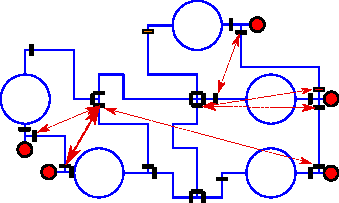
\includegraphics[width=2in,height=3in]{Fig/RA30_DFS.eps}
%\input{Fig/RA30_DFS.pdf_tex}
%\caption{DFT architecture and valve sharing of RA30.}
%\label{fig:RA30_DFT}
%}
%\end{figure}
%
%Finally, the DFT architecture with valve sharing of RA30 chip is shown in
%\figname~\ref{fig:RA30_DFT}. The red valve and channels are those inserted for
%DFT for single-source single-meter test.
%The valves connected by thin lines share the same control channels. As can be
%seen, it is even possible that more than two valves share a control channel in
%this case.
